\documentclass[conference]{IEEEtran}
\IEEEoverridecommandlockouts
% The preceding line is only needed to identify funding in the first footnote. If that is unneeded, please comment it out.
%Template version as of 6/27/2024

\usepackage{cite}
\usepackage{amsmath,amssymb,amsfonts}
\usepackage{algorithmic}
\usepackage{graphicx}
\usepackage{textcomp}
\usepackage{xcolor}
\usepackage{url}
\usepackage{enumitem}
\usepackage{subcaption}
\def\BibTeX{{\rm B\kern-.05em{\sc i\kern-.025em b}\kern-.08em
    T\kern-.1667em\lower.7ex\hbox{E}\kern-.125emX}}

\newcommand{\groupcap}{\texttt{group\_cap}}
\newcommand{\groupcapreq}{\texttt{group\_cap\_req}}
\newcommand{\groupupdate}{\texttt{group\_update}}
\newcommand{\groupreq}{\texttt{group\_req}}
\newcommand{\channelupdate}{\texttt{channel\_update}}
\newcommand{\groupsize}{\texttt{group\_size}}
\newcommand{\mincaplimit}{\texttt{min\_cap\_limit}}
\newcommand{\maxcaplimit}{\texttt{max\_cap\_limit}}

\begin{document}

\title{Routing Method Resolving Privacy-Latency Dilemma in Payment Channel Networks}

\author{\IEEEauthorblockN{Kohei Sato}
	\IEEEauthorblockA{\textit{Graduate School of Engineering and Science} \\
		\textit{Shibaura Institute of Technology}\\
		Tokyo, Japan \\
		af20023@shibaura-it.ac.jp}
	\and
	\IEEEauthorblockN{Hiroaki Morino}
	\IEEEauthorblockA{\textit{Graduate School of Engineering and Science} \\
		\textit{Shibaura Institute of Technology}\\
		Tokyo, Japan \\
		morino@shibaura-it.ac.jp}
}

\maketitle

\begin{abstract}
	We propose the Group Capacity Broadcast (GCB) method that discloses only the minimum capacity among grouped payment channels, thereby reducing payment retries while preserving privacy. Simulation results on a real Lightning Network snapshot show that GCB shortens payment confirmation delay compared with the conventional method without sacrificing success rate.
\end{abstract}

\begin{IEEEkeywords}
	Blockchain, Payment Channel Network, Routing Method, Gossip Protocol
\end{IEEEkeywords}

\section{Introduction}

In recent years, Payment Channel Networks (PCN)~\cite{poon_dryja_2016}, which connect multiple payment channels, have gained attention as solutions to blockchain~\cite{nakamoto2008bitcoin} scalability problems.

In a payment channel, two participants who intend to transact contribute sufficient funds for future transactions and send them to a blockchain address using transactions that can only be unlocked with the consensus of all participants. The total amount of contributed funds is called the channel capacity, and this value is publicly disclosed on the blockchain. Payments within a payment channel are executed by changing each participant's balance, but these changes are not recorded on the blockchain, enabling instant payment settlement.

A network constructed by connecting multiple payment channels is called a Payment Channel Network (PCN). In PCN, senders can safely and quickly transfer funds to recipients they are not directly connected to through multiple PCs using script-based transactions called HTLCs~\cite{poon_dryja_2016}. Furthermore, PCN not only process payments at high speed but also offer unique features not available in blockchains: since balances between payment channel participants are not publicly disclosed, payment information such as sender, recipient, and payment amount can be concealed from unrelated third parties.

When modeling PCN users as nodes in a directed graph and payment channels as bidirectional links between nodes, the balance of each upstream node corresponds to the link capacity in that direction, while transaction fees correspond to link costs, since it is impossible to send amounts exceeding the upstream node's balance in each direction of each payment channel. Unlike conventional communication networks, link capacity in each direction of a payment channel represents each participant's share of the initially contributed funds, so their sum always equals the channel capacity and remains constant, with each direction's capacity changing every time a payment is made. Additionally, since link capacity corresponds to the balance between participants within a payment channel, it is not disclosed to parties other than the participants themselves. Therefore, senders cannot accurately determine link capacities and must decide payment routes and attempt payments without considering link capacity, repeatedly retrying with alternative payment routes each time a payment fails.

This creates a fundamental dilemma where payment channels move most transactions off-chain to scale blockchains~\cite{poon_dryja_2016}, but senders must choose paths whose every link has enough capacity (i.e., upstream balance).

Here a dilemma arises.  If each link publicly reveals its current balance, the sender can pick a feasible path on the first try, but privacy is lost because observers can trace payments.  If balances remain secret, privacy is kept, yet the sender learns feasibility only after the attempt, causing expensive retries and long delays.  Lightning Network's~\cite{lnbolt} probabilistic routing slightly mitigates the delay but still struggles with large amounts.

This paper tackles the privacy–latency dilemma.  We evaluate the Group Capacity Broadcast (GCB) method, which discloses only the minimum balance inside a link group, thereby hiding individual balances while allowing the sender to rule out hopeless paths in advance.

\section{GCB Method}

GCB groups links with similar capacities and broadcasts only the minimum capacity within each group. A group constructor recruits links by broadcasting \groupreq{} messages specifying capacity range [\mincaplimit{}, \maxcaplimit{}]. Once \groupsize{} links join, the group must securely calculate its minimum capacity without exposing individual link balances.

The key innovation lies in a privacy-preserving minimum value computation protocol. Each group member initiates a \groupcap{} message containing its actual capacity and a unique identifier, which circulates through the group in a ring topology. As the message traverses each node, the capacity value is updated only if the current node's capacity is smaller, ensuring the final result represents the true minimum. To prevent observers from correlating capacity changes with specific links, nodes randomly abstain from updating the message approximately half the time during circulation. When a node receives its own message identifier after completing the full circuit, it recognizes the validity of the minimum value and broadcasts it network-wide as a \groupupdate{} message. This distributed consensus mechanism ensures that no single node can determine which link actually holds the minimum capacity, thereby maintaining payment privacy. Figure~\ref{fig:group_cap_handover} illustrates the detailed message flow of this protocol.

For routing decisions, senders can now determine path feasibility before transmission since each link's true capacity exceeds the disclosed group capacity. Senders use group capacity for grouped links and channel capacity for ungrouped links, applying standard shortest-path algorithms~\cite{lnd,eclair,clightning}. After successful payments, affected groups recalculate their minimum capacity to reflect balance changes, maintaining accuracy while preserving anonymity.

Privacy is preserved because observers cannot determine which specific link caused a group capacity change. Groups close when capacity updates exceed the initial range, triggering reformation with updated parameters to adapt to changing network conditions.

\begin{figure}[htbp]
	\centerline{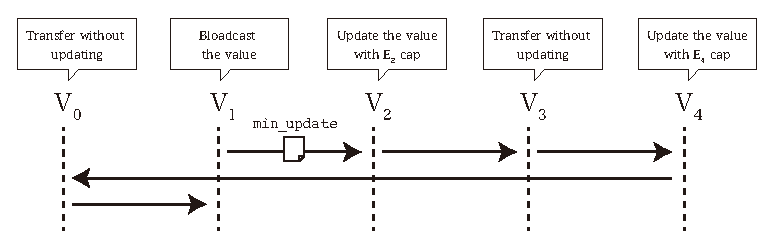
\includegraphics[width=\linewidth]{fig/group_cap_handover}}
	\caption{Group Capacity Calculation Protocol Message Flow}
	\label{fig:group_cap_handover}
\end{figure}

\section{Performance Evaluation}

This section evaluates the latency performance of the proposed GCB method using simulation.

\subsection{Evaluation Method}

We extended the payment channel network simulator CLoTH~\cite{CONOSCENTI2021100717}, which accurately reproduces Lightning Network HTLCs, implementing the GCB method.

We used a Lightning Network snapshot from December 17, 2020, with 6005 nodes and 60913 links. This data was obtained from LND's \texttt{describegraph} command, containing all publicly available information identical to the actual network. Since initial PC balances are undisclosed, we set them using uniformly distributed random numbers. We performed 5000 payments with amounts following normal distribution (mean $\mu = 10000$ sats, variance $\sigma = \mu \times 0.1$) and uniformly distributed random sender/recipient selection.

\subsection{Latency Evaluation}

Using optimal parameters $\groupsize=10, \alpha=0.1$, we compared GCB and LN methods for varying average payment amounts. Results show that while LN method confirmation delays increase significantly with payment amount, GCB method delays increase relatively little. For large payments, LN method experiences many retries due to considering only failure frequency without link capacity, prolonging confirmation time. GCB method eliminates unnecessary retries by disclosing group capacity, enabling immediate pre-send determination of impossible payments and minimizing confirmation delay increases even for large amounts, as demonstrated in Fig.~\ref{fig:pmt_amt_vs_time}.

\begin{figure}[htbp]
	\centerline{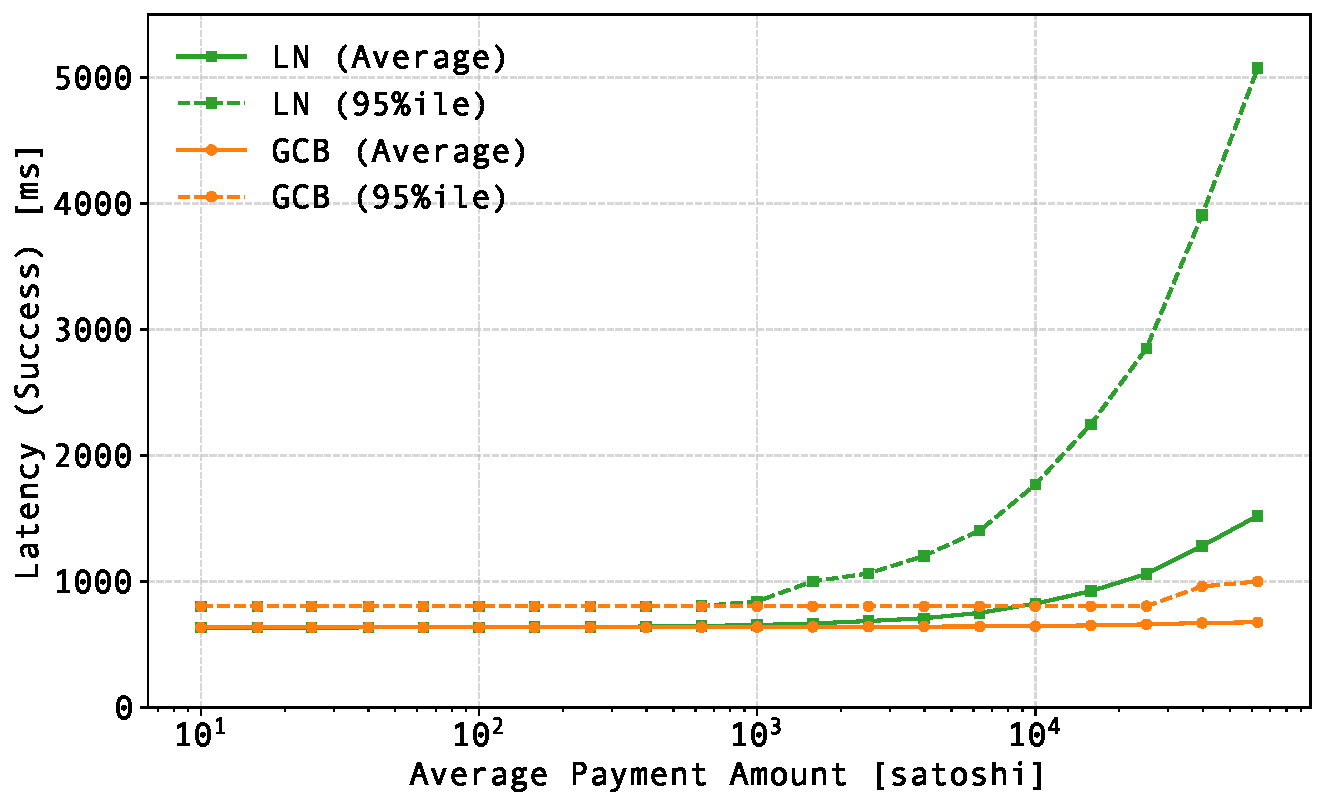
\includegraphics[width=\linewidth]{fig/pmt_amt_vs_time}}
	\caption{Latency of Sending Payment vs Payment Amount for Successful Cases Only}
	\label{fig:pmt_amt_vs_time}
\end{figure}

\section{Conclusion}

Simulation results confirmed that the proposed GCB method considerably shortens payment confirmation delay while maintaining a high success rate. Future work includes verifying payment information confidentiality under more diverse attack models.

\begin{thebibliography}{00}
	\bibitem{poon_dryja_2016} J. Poon and T. Dryja, ``The bitcoin lightning network: Scalable off-chain instant payments,'' 2016.
	\bibitem{nakamoto2008bitcoin} S. Nakamoto, ``Bitcoin: A peer-to-peer electronic cash system,'' 2008.
	\bibitem{lnbolt} ``BOLT: Basis of Lightning Technology,'' \url{https://github.com/lightningnetwork/lightning-rfc}.
	\bibitem{lnd} ``Lightning Network Daemon,'' \url{https://github.com/lightningnetwork/lnd}.
	\bibitem{clightning} ``Core Lightning,'' \url{https://github.com/ElementsProject/lightning}.
	\bibitem{eclair} ``Eclair,'' \url{https://github.com/ACINQ/eclair}.
	\bibitem{Andreescu_2021} O. Andreescu et al., ``Optimizing payment routing in the lightning network,'' in Proc. IEEE INFOCOM, 2021.
	\bibitem{published_papers/48227240} K. Sato and H. Morino, ``Group capacity broadcast method for payment channel networks,'' Technical Report, 2023.
	\bibitem{CONOSCENTI2021100717} M. Conoscenti et al., ``CLoTH: A simulator for HTLC payment networks,'' Future Generation Computer Systems, vol. 118, pp. 1--17, 2021.
\end{thebibliography}

\end{document}
